\chapter{Solvers}

In this chapter, all linear solvers are presented. Most of the iterative solvers can be performed on linear operators \emph{LocalMatrix}, \emph{LocalStencil} and \emph{GlobalMatrix} -- i.e. the iterative solvers can be performed locally (on a shared memory system) or in a distributed manner (on a cluster) via MPI. The only exception is the AMG (Algebraic Multigrid) which has two versions (one for the Local and one for the Global type of computation). The only pure local solvers (the one which does not support global/MPI operations) are the mixed-precision defect-correction solver, all direct solvers and the eigenvalue solvers.

All solvers need three template parameters -- Operators, Vectors and Scalar type. There are three possible combinations
\begin{itemize}
\itemsep0em
 \item \emph{LocalMatrix}, \emph{LocalVector}, \emph{float} or \emph{double}
 \item \emph{LocalStencil}, \emph{LocalVector}, \emph{float} or \emph{double}
 \item \emph{GlobalMatrix}, \emph{GlobalVector}, \emph{float} or \emph{double}
\end{itemize}

where the Operators/Vectors need to use the same ValueType as the scalar for the solver.

\section{Code Structure}

\begin{figure}[!ht]
\centering
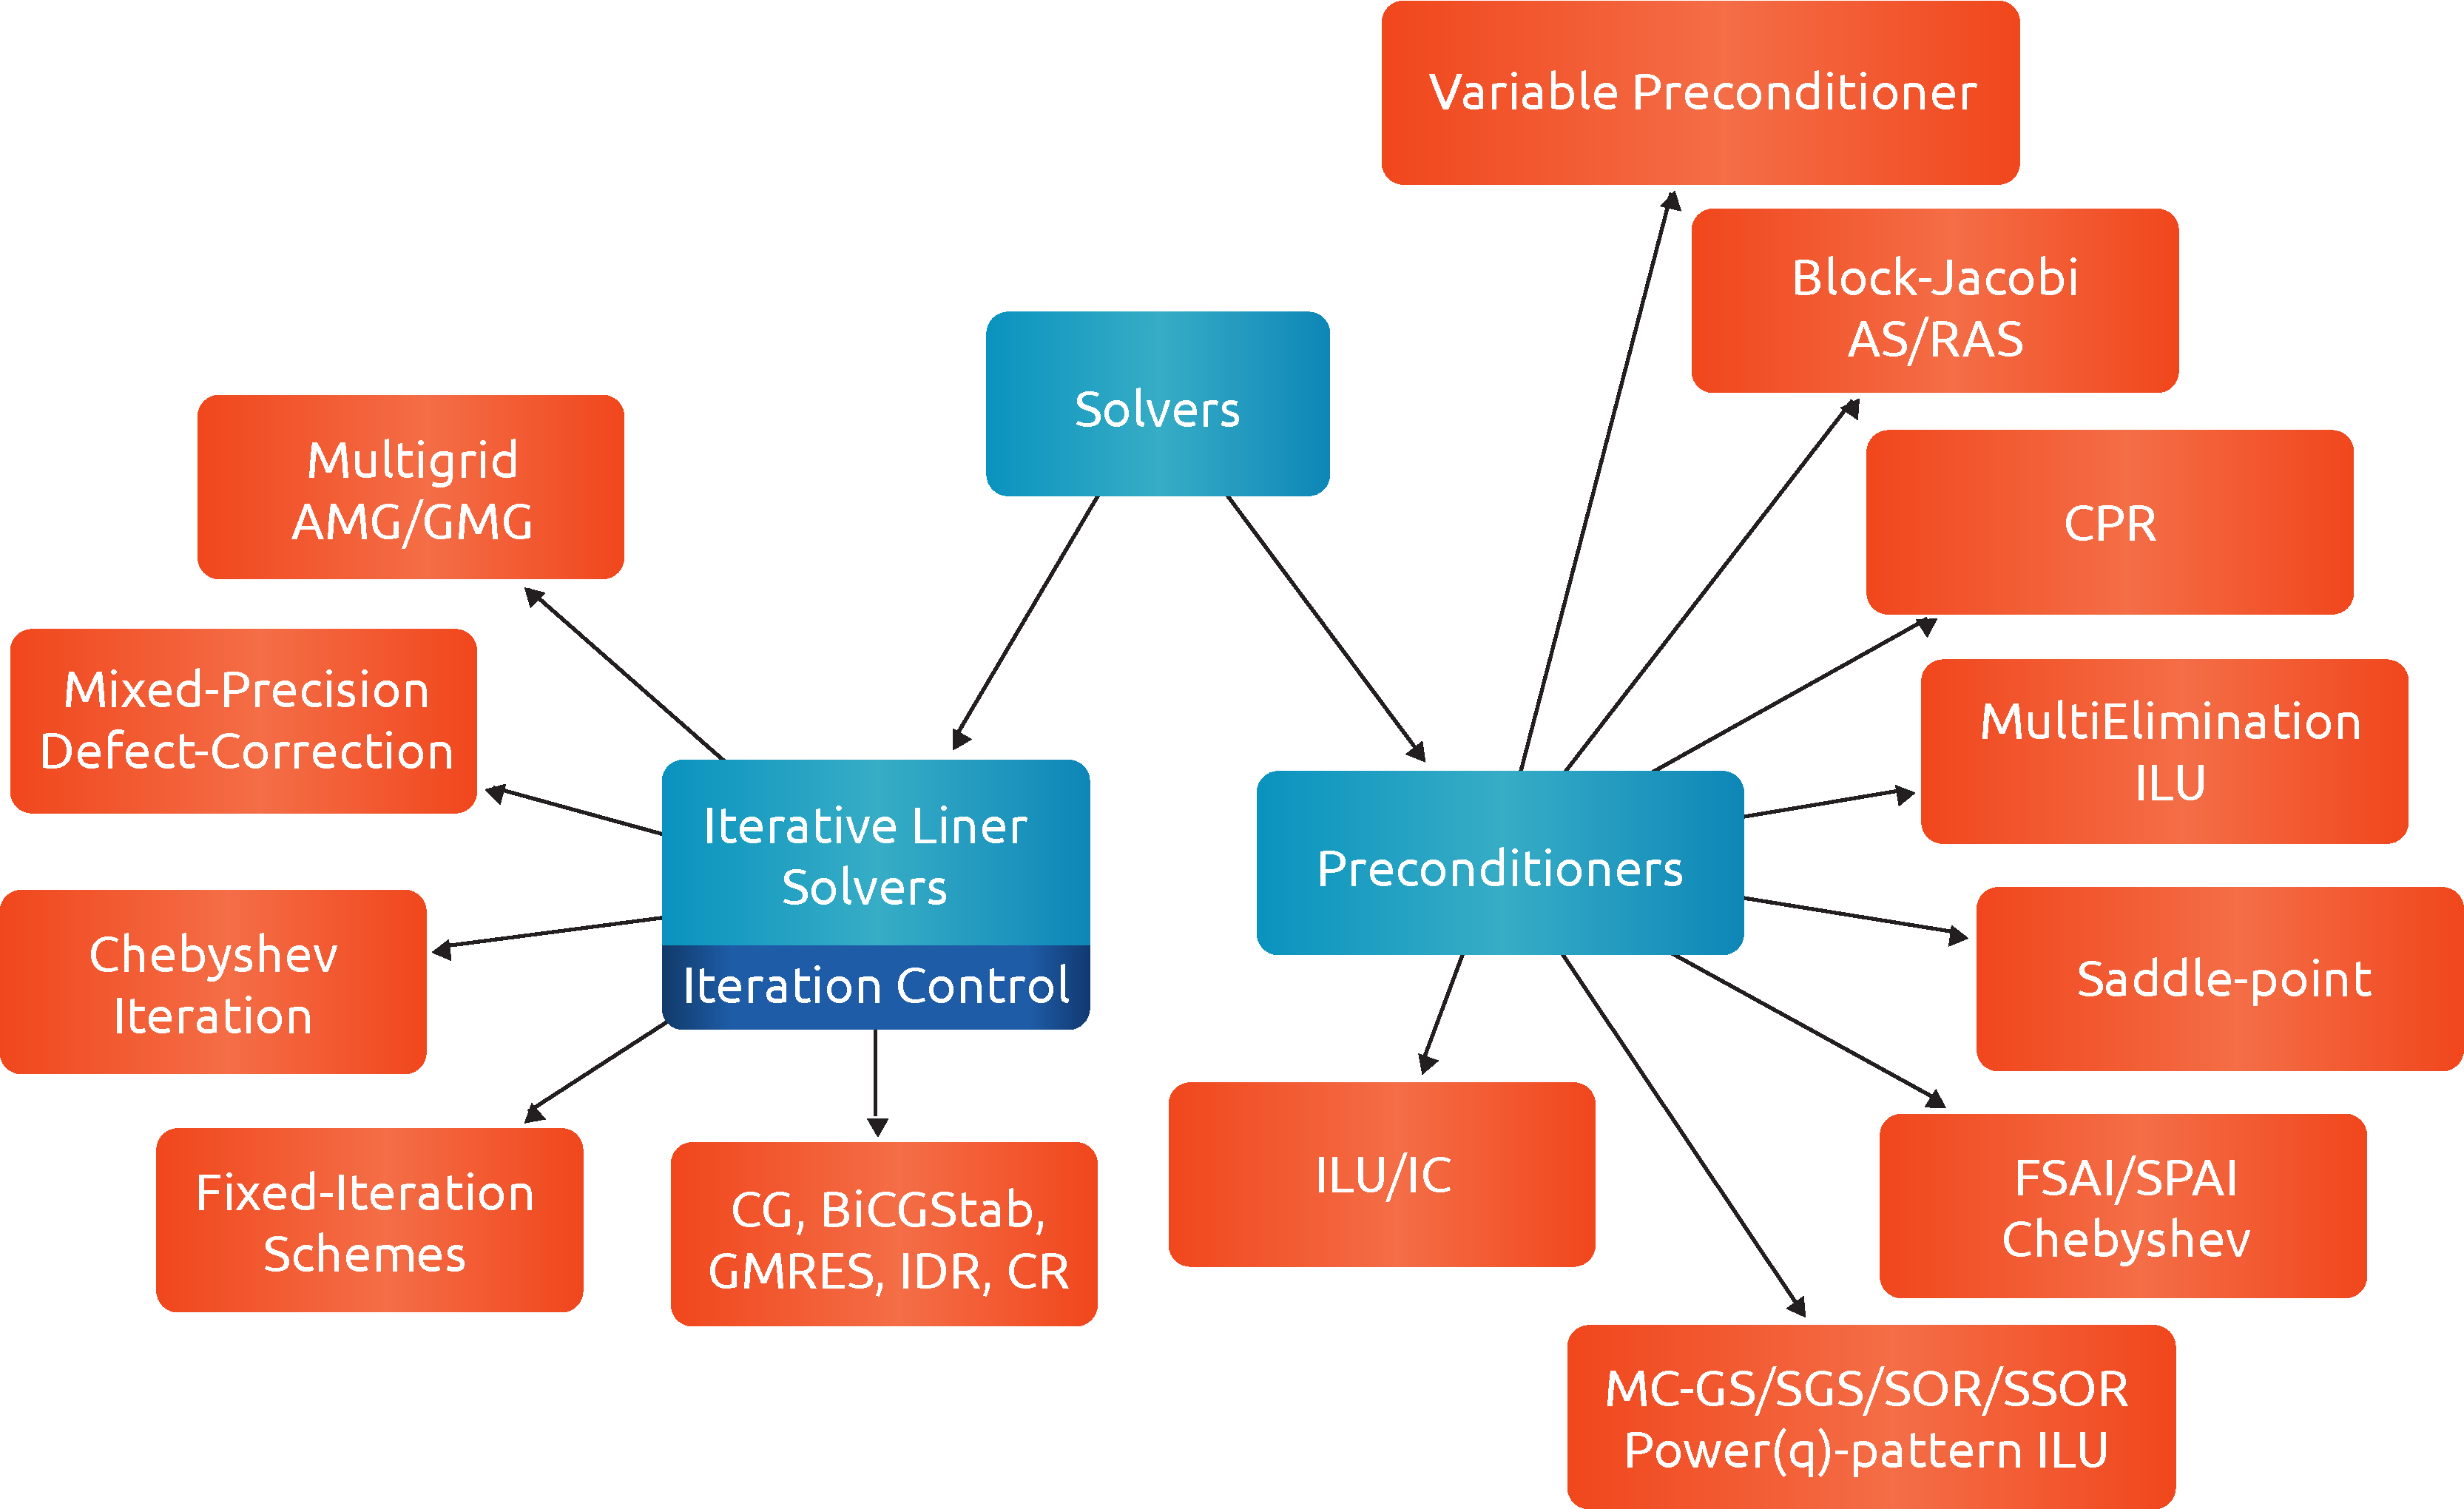
\includegraphics[width=0.95\textwidth]{./fig/solver.pdf}
\caption{Solver's classes hierarchy}
\label{paralution-solvers}
\end{figure}


The base class Solver is purely virtual, it provides an interface for:

\begin{itemize}
\itemsep0em
\item \emph{SetOperator()} -- set the operator $A$ - i.e. the user can pass the matrix here
\item \emph{Build()} -- build the solver (including preconditioners, sub-solvers, etc), the user need to specify the operator first
\item \emph{Solve()} -- solve the system $Ax=b$, the user need to pass a right-hand-side $b$ and a vector $x$ where the solution will be obtained
\item \emph{Print()} -- shows solver information
\item \emph{ReBuildNumeric()} -- only re-build the solver numerically (if possible), \item \emph{MoveToHost()} and \emph{MoveToAccelerator()} -- offload the solver (including preconditioners and sub-solvers) to the host/accelerator.
\end{itemize}

The computation of the residual can be based on different norms ($L_1$, $L_2$ and $L_{\infty}$). This is controlled by the function \emph{SetResidualNorm()}.


\begin{figure}[!ht]
\centering
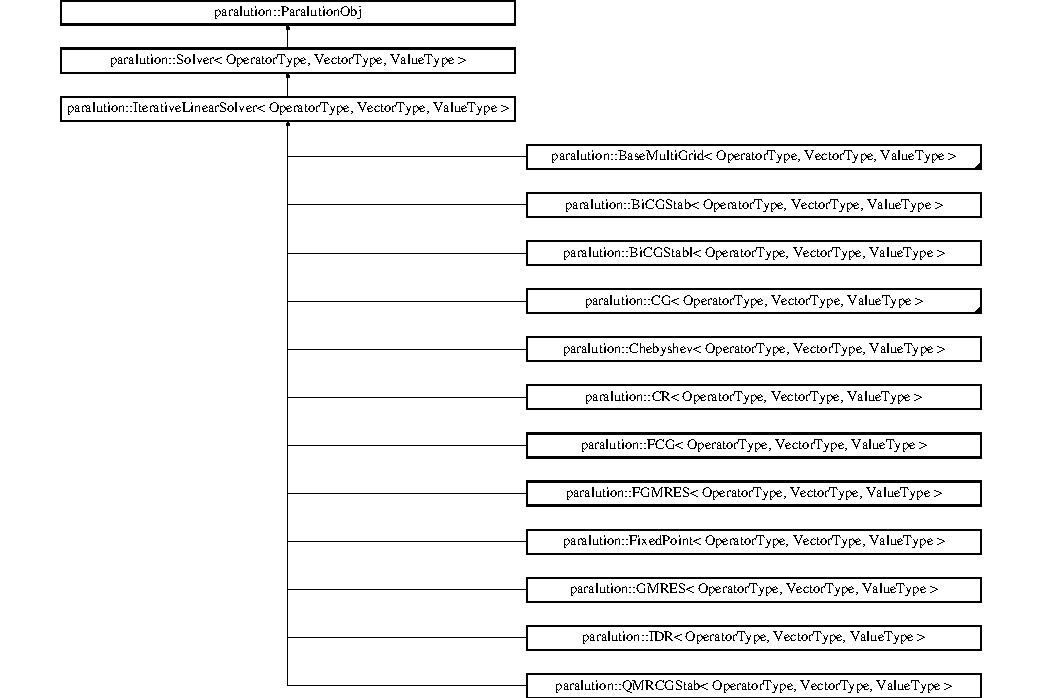
\includegraphics[width=0.8\textwidth]{./fig/body/classparalution_1_1_iterative_linear_solver.pdf}
\caption{Iterative Solvers}
\end{figure}

\begin{figure}[!ht]
\centering
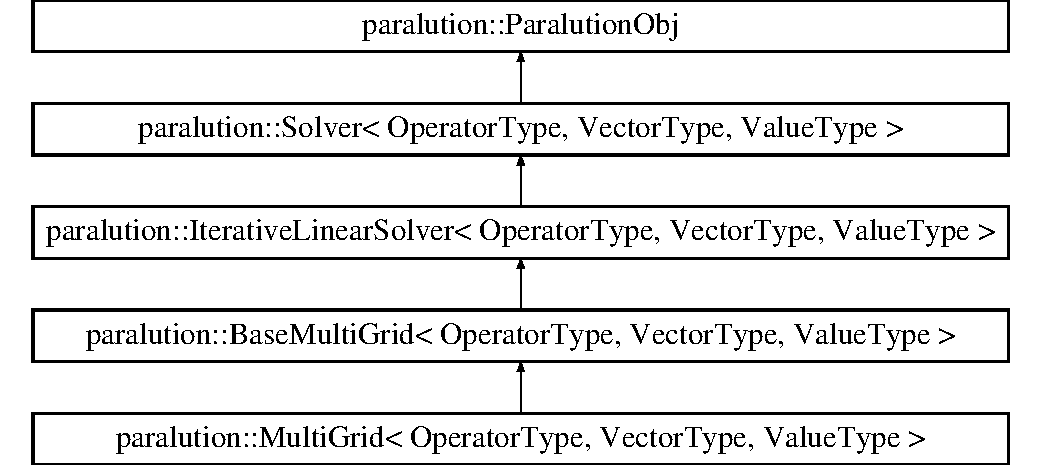
\includegraphics[width=0.5\textwidth]{./fig/body/classparalution_1_1_multi_grid.pdf}
\caption{Multi-Grid}
\end{figure}

\begin{figure}[!ht]
\centering
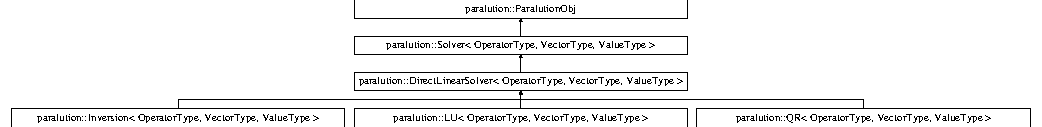
\includegraphics[width=0.9\textwidth]{./fig/body/classparalution_1_1_direct_linear_solver.pdf}
\caption{Direct Solvers}
\end{figure}


\section{Iterative Linear Solvers}

The iterative solvers are controlled by an iteration control object, which monitors the convergence properties of the solver - i.e. maximum number of iteration, relative tolerance, absolute tolerance, divergence tolerance. The iteration control can also record the residual history and store it in an ASCII file.

\begin{itemize}
\itemsep0em
\item \emph{Init()}, \emph{InitMinIter()}, \emph{InitMaxIter()}, \emph{InitTol()} -- initialize the solver and set the stopping criteria
\item \emph{RecordResidualHistory()}, \emph{RecordHistory()} -- start the recording of the residual and store it into a file
\item \emph{Verbose()} -- set the level of verbose output of the solver (0 -- no output, 2 -- detailed output, including residual and iteration information)
\item \emph{SetPreconditioner()} -- set the preconditioning
\end{itemize}

\section{Stopping Criteria}

All iterative solvers are controlled based on:
\begin{itemize}
\itemsep0em
\item Absolute stopping criteria, when the $|r_k|_{L_p} < eps_{ABS}$
\item Relative stopping criteria, when the $|r_k|_{L_p} / |r_1|_{L_p} \leq eps_{REL}$ 
\item Divergence stopping criteria, when the $|r_k|_{L_p} / |r_1|_{L_p} \geq eps_{DIV}$
\item Maximum number of iteration $N$, when $k = N$ 
\end{itemize}

where $k$ is the current iteration, $r_k$ is the residual for the current iteration $k$ (i.e. $r_k=b-A x_k$), $r_1$ is the starting residual (i.e. $r_1=b-Ax_{initguess}$).
In addition, the minimum number of iteration $M$ can be specified. In this case, the solver will not stop to iterate before $k \geq M$.

\lstinputlisting[title="Setting different stopping criteria in a CG solver"]{./src/cg.cpp}


The $L_p$ is the norm used for the computation, where $p$ could be $1$, $2$ and $\infty$. The norm computation can be set via \emph{SetResidualNorm()} function with 1 for $L_1$, 2 for $L_2$ and 3 for $L_{\infty}$. For the computation with the $L_{\infty}$, the index of maximum value can be obtained via the \emph{GetAmaxResidualIndex()} function. If this function is called and the $L_{\infty}$ has not been selected then this function will return $-1$.

The reached criteria can be obtained via \emph{GetSolverStatus()}, which will return:

\begin{itemize}
\itemsep0em
\item 0 -- if no criteria has been reached yet
\item 1 -- if absolute tolerance has been reached
\item 2 -- if relative tolerance has been reached
\item 3 -- if divergence tolerance has been reached
\item 4 -- if maximum number of iteration has been reached
\end{itemize}

\lstinputlisting[title="CG solver with $L_1$ norm"]{./src/cg-L1.cpp}
\lstinputlisting[title="CG solver with $L_{\infty}$ norm"]{./src/cg-Linf.cpp}

\section{Building and Solving Phase}

Each iterative solver consists of a building step and a solving step. During the building step all necessary auxiliary data is allocated and the preconditioner is constructed. After that the user can call the solving procedure, the solving step can be called several times. 

When the initial matrix associated with the solver is on the accelerator, the solver will try to build everything on the accelerator. However, some preconditioners and solvers (such as FSAI and AMG) need to be constructed on the host and then they are transferred to the accelerator. If the initial matrix is on the host and we want to run the solver on the accelerator then we need to move the solver to the accelerator as well as the matrix, the right-hand-side and the solution vector. Note that if you have a preconditioner associate with the solver, it will be moved automatically to the accelerator when you move the solver. In the following Listing we present these two scenarios.

\lstinputlisting[title="An example for a preconditioend CG where the building phase and the solution phase are performed on the accelerator"]{./src/solver-accel.cpp}

\lstinputlisting[title="An example for a preconditioned CG where the building phase is performed on the host and the solution phase is performed on the accelerator"]{./src/solver-accel2.cpp}

\section{Clear function and Destructor}

The \emph{Clear()} function clears all the data which is in the solver including the associated preconditioner. Thus, the solver is not anymore associated with this preconditioner. Note that the preconditioner is not deleted (via destructor) only a \emph{Clear()} is called.

When the destructor of the solver class is called, it automatically call the \emph{Clear()} function. Be careful, when declaring your solver and preconditioner in different places - we highly recommend to manually call the \emph{Clear()} function of the solver and not to relay on destructor of the solver.

\section{Numerical Update}

\begin{table}[H]
\begin{tabular}{l|l|l}
\multicolumn{1}{c|}{ValueType} & Building phase & Available \\ \hline
D,F,C                          & H,C            & S,M      
\end{tabular}
\end{table}

Some preconditioners require two phases in the their construction: an algebraic (e.g. compute a pattern or structure) and a numerical (compute the actual values). In cases, where the structure of the input matrix is a constant (e.g. Newton-like methods) it is not necessary to fully re-construct the preconditioner. In this case, the user can apply a numerical update to the current preconditioner and passed the new operator. 

This function is called \emph{ReBuildNumeric()}. If the preconditioner/solver does not support the numerical update, then a full \emph{Clear()} and \emph{Build()} will be performed.

\section{Fixed-point Iteration}


Fixed-point iteration is based on additive splitting of the matrix as $A=M+N$, the scheme reads
%
\begin{eqnarray}
 x_{k+1}=M^{-1}(b-N x_{k}).
\end{eqnarray}

It can also be reformulated as a weighted defect correction scheme 
\begin{equation}
 x_{k+1}=x_{k} - \omega M^{-1}(Ax_{k}-b).
\end{equation}

The inversion of $M$ can be performed by preconditioners (Jacobi, Gauss-Seidel, ILU, etc) or by any type of solvers. 

\begin{table}[H]
\begin{tabular}{l|l|l|l}
\multicolumn{1}{c|}{ValueType} & Building phase & Solving phase & Available \\ \hline
D,F,C                          & H,C,O,X        & H,C,O,X       & S,M      
\end{tabular}
\end{table}

\lstinputlisting[title="Fixed-Point declaration"]{./dec/fp.cpp}


\lstinputlisting[title="Fixed-point iteration based on Jacobi preconditioner - Jacobi iteration"]{./src/fp.cpp}


\section{Krylov Subspace Solvers}

Krylov subspace solvers are iterative methods based on projection. The implemented solvers in PARALUTION are CG, CR, BiCGStab, BiCGStab(l), QMRCGStab, GMRES, as well as Flexible CG and Flexible GMRES. Details of the methods can be found in \cite{SAAD, templates, Demmel, IDR1, IDR2}.

\subsection{CG}

CG (Conjugate Gradient) is a method for solving symmetric and positive definite matrices (SPD). The method can be preconditioned where the approximation should also be SPD.


\begin{table}[H]
\begin{tabular}{l|l|l|l}
\multicolumn{1}{c|}{ValueType} & Building phase & Solving phase & Available \\ \hline
D,F,C                          & H,C,O,X        & H,C,O,X       & S,M      
\end{tabular}
\end{table}

\lstinputlisting[title="CG declaration"]{./dec/cg.cpp}


\subsection{CR}

CR (Conjugate Residual) is a method for solving symmetric and semi-positive definite matrices. The method can be preconditioned where the approximation should also be SPD or semi-SPD.


\begin{table}[H]
\begin{tabular}{l|l|l|l}
\multicolumn{1}{c|}{ValueType} & Building phase & Solving phase & Available \\ \hline
D,F,C                          & H,C,O,X        & H,C,O,X       & S,M      
\end{tabular}
\end{table}


\lstinputlisting[title="CR declaration"]{./dec/cr.cpp}

\subsection{GMRES}

GMRES (Generalized Minimal Residual Method) is a method for solving non-symmetric problems. The pure GMRES solvers is based on restarting technique. The default size of the Krylov subspace for the GMRES is set to 30, it can be modify by \emph{SetBasisSize()} function.

\begin{table}[H]
\begin{tabular}{l|l|l|l}
\multicolumn{1}{c|}{ValueType} & Building phase & Solving phase & Available \\ \hline
D,F,C                          & H,C,O,X        & H,C,O,X       & S,M      
\end{tabular}
\end{table}


\lstinputlisting[title="GMRES declaration"]{./dec/gmres.cpp}


\subsection{FGMRES}

FGMRES (Flexible Generalized Minimal Residual Method) is a method for solving non-symmetric problems. The Flexible GMRES solvers is based on a window shifting of the Krylov subspace. The default size of the Krylov subspace for the GMRES is set to 30, it can be modify by \emph{SetBasisSize()} function.


\begin{table}[H]
\begin{tabular}{l|l|l|l}
\multicolumn{1}{c|}{ValueType} & Building phase & Solving phase & Available \\ \hline
D,F,C                          & H,C,O,X        & H,C,O,X       & S,M      
\end{tabular}
\end{table}


\lstinputlisting[title="FGMRES declaration"]{./dec/fgmres.cpp}

\subsection{BiCGStab}

BiCGStab (Bi-Conjugate Gradient Stabilized) is a method for solving non-symmetric problems.

\begin{table}[H]
\begin{tabular}{l|l|l|l}
\multicolumn{1}{c|}{ValueType} & Building phase & Solving phase & Available \\ \hline
D,F,C                          & H,C,O,X        & H,C,O,X       & S,M      
\end{tabular}
\end{table}

\lstinputlisting[title="BiCGStab declaration"]{./dec/bicgstab.cpp}



\subsection{IDR}

IDR (Induced Dimension Reduction) is a method for solving non-symmetric problems. The dimension of the shadow space for the IDR($s$) method can be set by \emph{SetShadowSpace()} function, the default value is $4$.

\begin{table}[H]
\begin{tabular}{l|l|l|l}
\multicolumn{1}{c|}{ValueType} & Building phase & Solving phase & Available \\ \hline
D,F,C                          & H,C,O,X        & H,C,O,X       & S,M      
\end{tabular}
\end{table}


\lstinputlisting[title="IDR Solver"]{./dec/idr.cpp}

\textbf{\emph{Note}} The orthogonal system in IDR method is based on random numbers, thus it is normal to obtain slightly different number of iterations every time you run the program.

\subsection{FCG}

FCG (Flexible Conjugate Gradient) is a method for solving symmetric and positive definite matrices (SPD). The method can be preconditioned where the approximation should also be SPD. For additional informations see~\cite{fcg}.

\begin{table}[H]
\begin{tabular}{l|l|l|l}
\multicolumn{1}{c|}{ValueType} & Building phase & Solving phase & Available \\ \hline
D,F,C                          & H,C,O,X        & H,C,O,X       & S,M      
\end{tabular}
\end{table}

\lstinputlisting[title="FCG declaration"]{./dec/fcg.cpp}

\subsection{QMRCGStab}

QMRCGStab is a method for solving non-symmetric problems. More details are given in~\cite{qmrcgstab}.

\begin{table}[H]
\begin{tabular}{l|l|l|l}
\multicolumn{1}{c|}{ValueType} & Building phase & Solving phase & Available \\ \hline
D,F,C                          & H,C,O,X        & H,C,O,X       & S,M      
\end{tabular}
\end{table}

\lstinputlisting[title="QMRCGStab declaration"]{./dec/qmrcgstab.cpp}

\subsection{BiCGStab(l)}

BiCGStab(l) (Bi-Conjugate Gradient Stabilized) is a method for solving non-symmetric problems. The degree $l$ can be set via the function \emph{SetOrder()}. More details can be found in~\cite{bicgstabl}.

\begin{table}[H]
\begin{tabular}{l|l|l|l}
\multicolumn{1}{c|}{ValueType} & Building phase & Solving phase & Available \\ \hline
D,F,C                          & H,C,O,X        & H,C,O,X       & S,M      
\end{tabular}
\end{table}

\lstinputlisting[title="BiCGStab(l) declaration"]{./dec/bicgstabl.cpp}

\subsection*{Example}

\lstinputlisting[title="Preconditioned CG solver with ILU($0$ $1$)"]{./src/cg1.cpp}

\section{Chebyshev Iteration}

The Chebyshev iteration (also known as acceleration scheme) is similar to the CG method but it requires the minimum and the maximum eigenvalue of the matrix. Additional information can be found in \cite{templates}.

\begin{table}[H]
\begin{tabular}{l|l|l|l}
\multicolumn{1}{c|}{ValueType} & Building phase & Solving phase & Available \\ \hline
D,F,C                          & H,C,O,X        & H,C,O,X       & S,M      
\end{tabular}
\end{table}

\lstinputlisting[title="Chebyshev iteration"]{./src/cheb.cpp}

\section{Mixed-precision Solver}

The library provides mixed-precision solvers based on defect-correction scheme. The current implementation of the library is based on host correction in double precision and accelerator computation in single precision. The solver is based on the following scheme:
%
\begin{eqnarray}
 x_{k+1}=x_{k} + A^{-1}r_{k},
\end{eqnarray}
%
where the computation of the residual $r_{k}=b-A x_{k}$ and of the update $ x_{k+1}=x_{k} + d_{k}$ are performed on the host in double precision. The computation of the residual system $Ad_k=r_k$ is performed on the accelerator in single precision. In addition to the setup functions of the iterative solver, the user need to specify the inner (for $Ad_k=r_k$) solver.

\begin{table}[H]
\begin{tabular}{l|l|l|l}
\multicolumn{1}{c|}{ValueType} & Building phase & Solving phase & Available \\ \hline
D-F                            & H,C,O,X        & H,C,O,X       & S,M      
\end{tabular}
\end{table}


\lstinputlisting[title="Mixed-precision solver"]{./src/mp.cpp}

\section{Multigrid Solver}

The library provides algebraic multigrid as well as a skeleton for geometric multigrid methods. The \emph{BaseMultigrid} class itself is not constructing the data for the method. It contains the solution procedure for V, W, K-cycles, for details see \cite{Trottenberg2003}. 

The AMG has two different versions for Local (non-MPI) and for Global (MPI) type of computations.

\subsection{Geometric Multigrid}

\begin{table}[H]
\begin{tabular}{l|l|l|l}
\multicolumn{1}{c|}{ValueType} & Building phase & Solving phase & Available \\ \hline
D,F,C                          & -              & H,C,O,X       & S,M      
\end{tabular}
\end{table}

For the geometric multgrid the user need to pass all information for each level and for its construction. This includes smoothing step, prolongation/restriction, grid traversing and coarsest level solver. This data need to be passed to the solver:

\begin{itemize}
\itemsep0em

\item Restriction and prolongation operations -- they can be performed in two ways, based on \emph{Restriction()} and \emph{Prolongation()} function of the LocalVector class, or by matrix-vector multiplication. This is configured by a set function.

\item Smoothers -- they can be of any iterative linear solver's type. Valid options are Jacobi, Gauss-Seidel, ILU, etc. using a FixedPoint iteration scheme with pre-defined number of iterations. The smoothers could also be a solver such as CG, BiCGStab, etc.

\item Coarse grid solver -- could be of any iterative linear solver type. The class also provides mechanisms to specify where the coarse grid solver has to be performed on the host or on the accelerator. The coarse grid solver can be preconditioned.

\item Grid scaling -- computed based on a L2 norm ratio.

\item Operator matrices - the operator matrices need to be passed on each grid level

\item All objects need to be passed already initialized to the multigrid class.

\end{itemize}

\subsection{Algebraic Multigrid}

\subsubsection{Plain and Smoothed Aggregation}

\begin{table}[H]
\begin{tabular}{l|l|l|l}
\multicolumn{1}{c|}{ValueType} & Building phase & Solving phase & Available \\ \hline
D,F,C                          & H              & H,C,O,X       & S,M      
\end{tabular}
\end{table}


The algebraic multigrid solver (AMG) is based on the \emph{Multigrid} class. The coarsening is obtained by different aggregation techniques. Currently, we support interpolation schemes based on aggregation~\cite{stuben} and smoothed aggregation~\cite{vanek}.  The smoothers could be constructed inside or outside of the class. Detailed examples are given in the examples section.

When building the AMG if not additional information is set, the solver is built based on its default values.
\lstinputlisting[title="AMG as a standalone solver"]{./src/amg.cpp}

All parameters can in the AMG can be set externally, including smoothers and coarse-grid solver - any type of solvers can be used.
\lstinputlisting[title="AMG with manual settings"]{./src/amg2.cpp}

The AMG can be used also as a preconditioner within a solver.
\lstinputlisting[title="AMG as a preconditioner"]{./src/cg_amg.cpp}

\subsubsection{Ruge-Stueben}

The classic Ruge-Stueben coarsening algorithm is implemented following the ~\cite{stuben}.

\begin{table}[H]
\begin{tabular}{l|l|l|l}
\multicolumn{1}{c|}{ValueType} & Building phase & Solving phase & Available \\ \hline
D,F,C                          & H              & H,C,O,X       & S,M      
\end{tabular}
\end{table}

The solver provides high-efficiency in terms of complexity of the solver (i.e. number of iterations). However, most of the time it has a higher building step and requires higher memory usage.


\subsubsection{Pair-wise}

The pairwise aggregation scheme is based on~\cite{pairwiseamg}.

\begin{table}[H]
\begin{tabular}{l|l|l|l}
\multicolumn{1}{c|}{ValueType} & Building phase & Solving phase & Available \\ \hline
D,F,C                          & H              & H,C,O,X       & S,M      
\end{tabular}
\end{table}

The pairwise AMG delivers very efficient building phase which is suitable for Poisson-like equation. Most of the time it requires K-cycle for the solving phase to provide low number of iterations.

\subsubsection{Global AMG (MPI)}

The global AMG is based on a variation of the pairwise aggregation scheme, using the MPI standard for inter-node communication.

\begin{table}[H]
\begin{tabular}{l|l|l|l}
\multicolumn{1}{c|}{ValueType} & Building phase & Solving phase & Available \\ \hline
D,F,C                          & H              & H,C,O,X       & M      
\end{tabular}
\end{table}

The building and the solving phase are fully MPI parallel. This solver works well with updating technique suitable for time-dependent problems (i.e. time-stepping schemes) which decrease significantly the building phase.


\section{Direct Linear Solvers}

The library provides three direct methods -- LU, QR and full inversion (based on QR decomposition). The user can pass a sparse matrix, internally it will be converted to dense and then the selected method will be applied. These methods are not very optimal and due to the fact that the matrix is converted in a dense format, these methods should be used only for very small matrices.

\lstinputlisting[title="A direct solver"]{./src/direct.cpp}

\textbf{\emph{Note}} These methods works only for Local-type of problems (no distributed problems).
